\section{Equations, Figures, and Tables}
연구 본문은 하위 절(subsection, subsubsection, ...)등이 등장하는 경우가 있다. 이 때는 {\textbackslash}subsection\{section name\}, {\textbackslash}subsubsection\{subsubsection name\}을 사용하여 하위 절을 구성하면 된다. 여기서는 수식 작성법, 그림 넣는 법, 표 만드는 법에 대해 살펴본다.

\subsection{Equations}

먼저 문장 속에서 수식을 사용하는 경우에는 \$ (수식) \$과 같이 처리하면 된다. 다음과 같이 작성한 후 컴파일을 하면
\begin{quote}
운동 에너지는 \$(1/2)mv$\wedge$2\$으로 표현된다. 여기서 \$m\$은 물체의 질량, \$v\$ 는 물체의 속력이다.
\end{quote}
pdf 파일에는 다음과 같이 나타난다.
\begin{quote}
운동 에너지는 $(1/2)mv^2$으로 표현된다. 여기서 $m$은 물체의 질량, $v$는 물체의 속력이다.
\end{quote}
위의 예시에서 보듯이 문장 속에서 수식을 사용할 때는 한 줄로 입력한다. 즉 분수 형태의 수식은 슬래쉬`/'로 대체하여 표현한다. 줄 간격을 일정하게 유지하기 위함이다.

다음은 수식이 문장 밖으로 나와 한 줄을 통째로 차지하는 경우이다. 수식을 작성하는 명령어는 다양하지만, 여기서는 equation, align에 대해서만 다룬다. 먼저 equation의 사용법을 예를 통해 확인해보자. 만약 다음과 같이 입력을 하고
\begin{lstlisting}
	\begin{equation}
	\int_V \nabla\cdot{\rm\bf F} dV = \oint_S {\rm\bf F}\cdot d{\rm\bf A}. \label{eq001}
	\end{equation}
\end{lstlisting}
컴파일을 하면 다음과 같은 식이 pdf파일에 나타나는 것을 확인할 수 있다.
\begin{equation}
\int_V \nabla\cdot{\rm\bf F} dV = \oint_S {\rm\bf F}\cdot d{\rm\bf A}. \label{eq001}
\end{equation}
문장 속에서 수식의 번호(라벨)을 호출하는 경우가 종종 있다. 이 때는 {\textbackslash}ref\{eq001\}을 사용하면 된다. 여기서 eq001은 수식에서 label 명령어 다음에 작성된 문구이다. 수식마다 각기 다른 라벨을 작성해야 하며 논문 저자가 기억하기 편한 것을 사용하면 된다. 서로 다른 수식에 중복된 라벨을 사용하면, 나중에 작성된 라벨의 수식 번호만 호출됨에 유의하라. 사용 예는 다음과 같다.
\begin{quote}
(작성 예) Divergence 이론은 임의의 벡터 필드 \${\textbackslash}rm{\textbackslash}bf F\$가 임의의 폐곡면 외부를 향하는 플럭스의 총량은 \${\textbackslash}nabla{\textbackslash}cdot\{{\textbackslash}rm{\textbackslash}bf F\}\$ 를 폐곡면 내부 부피에 대하여 적분한 것과 같다는 것으로 이를 식으로 표현하면 식 ({\textbackslash}ref\{eq001\}) 과 같다.
\end{quote}
\begin{quote}
(컴파일 결과) Divergence 이론은 임의의 벡터 필드 $\rm\bf F$가 임의의 폐곡면 외부를 향하는 플럭스의 총량은 $\nabla\cdot{\rm\bf F}$를 폐곡면 내부 부피에 대하여 적분한 것과 같다는 것으로 이를 식으로 표현하면 식 (\ref{eq001})과 같다.
\end{quote}
그런데 수식에 번호를 붙일 필요가 없는 경우도 있다. 이 경우에는 수식이 끝나고 equation 명령어를 닫기 전 {\textbackslash}nonumber라고 입력하면 된다.
\begin{lstlisting}
	\begin{equation}
	\pi=3.14159265358979... \nonumber
	\end{equation}
\end{lstlisting}
\begin{equation}
\pi=3.14159265358979... \nonumber
\end{equation}
지금까지 equation 명령어에 대해 살펴보았는데, equation은 한 줄로 표현 가능한 수식에 사용된다. 그런데 수식 중에는 한 줄로 표현하기 너무 길어서 줄바꿈을 해야 할 필요가 있는 경우, 또는 여러 줄에 걸쳐서 계산 과정을 보여줄 필요가 있는 경우가 있다. 이 때 사용되는 대표적인 명령어가 align이다.
\begin{lstlisting}
	\begin{align}
	\frac{dE}{dt} &=\frac{\partial E}{\partial t} +\sum_i \dot{q}_i \frac{\partial E}{\partial q_i} +\sum_i \ddot{q}_i \frac{\partial E}{\partial\dot{q}_i} \notag\\
	&=\sum_j \dot{q}_j \sum_k \left( A_{jk} q_k +M_{jk} \ddot{q}_k \right). \label{eq002}
	\end{align}
\end{lstlisting}
\TeX\ 파일에 위와 같이 입력하고 컴파일을 해보면 다음과 같은 식을 얻는다.
\begin{align}
\frac{dE}{dt} &=\frac{\partial E}{\partial t} +\sum_i \dot{q}_i \frac{\partial E}{\partial q_i} +\sum_i \ddot{q}_i \frac{\partial E}{\partial\dot{q}_i} \notag\\
&=\sum_j \dot{q}_j \sum_k \left( A_{jk} q_k +M_{jk} \ddot{q}_k \right). \label{eq002}
\end{align}
\TeX\ 파일에 입력된 등호 앞의 \& 기호는 줄 맞춤 표시이다. 즉, 첫 번째 줄의 \&와 두 번째 줄의 \&가 같은 수직선상에 위치한다는 의미이다. 첫 번째 줄에서는 수식 번호를 넣고 싶지 않아서 {\textbackslash}notag라는 명령어를 사용하였다. equation 명령어에서 사용된 {\textbackslash}nonumber와 같은 기능을 한다. 줄을 넘길 때는 {\textbackslash}{\textbackslash}를 사용한다. 이번에는 줄이 너무 길어서 여러 줄에 나누어 표현하는 식의 예를 살펴보자. (P. H. Yoon의 2006 논문에서 참고하였음 \cite{Yoon06})
\begin{lstlisting}
	\begin{align}
	\delta P_{ij}^a =&\frac{i}{B_0} \frac{\Omega_a}{\omega-{\rm\bf k}\cdot{\rm\bf v}_a} \left( m_a n \epsilon_{ikl} v_k^a B_l \delta v_j^a +m_a n \epsilon_{jkl} v_k^a B_l \delta v_i^a \right. \notag\\
	&\left. +\epsilon_{ikl} \delta B_l P_{jk}^a +\epsilon_{jkl} \delta B_l P_{ik}^a +\epsilon_{ikl} B_l \delta P_{jk}^a +\epsilon_{jkl} B_l \delta P_{ik}^a \right) . \label{eq003}
	\end{align}
\end{lstlisting}
위와 같이 작성한 후 컴파일하면 pdf 파일에 다음과 같은 식이 등장한다.
\begin{align}
\delta P_{ij}^a =&\frac{i}{B_0} \frac{\Omega_a}{\omega-{\rm\bf k}\cdot{\rm\bf v}_a} \left( m_a n \epsilon_{ikl} v_k^a B_l \delta v_j^a +m_a n \epsilon_{jkl} v_k^a B_l \delta v_i^a \right. \notag\\
&\left. +\epsilon_{ikl} \delta B_l P_{jk}^a +\epsilon_{jkl} \delta B_l P_{ik}^a +\epsilon_{ikl} B_l \delta P_{jk}^a +\epsilon_{jkl} B_l \delta P_{ik}^a \right) . \label{eq003}
\end{align}
보는 바와 같이 괄호 내부가 너무 길어서 줄바꿈을 했더니 첫 줄에서 괄호가 열리고 다음 줄에서 괄호가 닫힌다. \TeX에서는 괄호를 연 뒤, 닫지 않고 줄바꿈을 하면 에러가 발생한다. 따라서 첫 줄에서 `{\textbackslash}left('로 괄호를 연 뒤, `{\textbackslash}right.'으로 괄호를 닫았다. 이 표시는 실제로 pdf 파일에는 등장하지 않지만 에러 방지를 위해 넣어준 것이다. 두 번째 줄에서도 마찬가지로 `{\textbackslash}left.'으로 (pdf 파일에는 보이지 않는) 괄호를 연 뒤 `{\textbackslash}right)'으로 괄호를 닫아주었다.

align 명령어는 각 줄마다 수식 번호가 작성 가능하다. 그래서 식 (\ref{eq003})과 같이 하나의 식을 두 줄에 나누어 표현할 때 (첫 번째 줄에는 notag 명령어를 넣어 수식 번호를 제거하고) 두 번째 줄에 수식 번호가 등장하도록 하였다. 그런데 이처럼 하나의 식을 여러 줄에 걸쳐 표현할 때는 수식 번호의 상하 위치가 수식 전체의 중앙에 등장하는 편이 더 보기 좋다. 이 경우에는 equation 명령어 내부에 다시 split 명령어를 사용하면 된다. 다음 식 (\ref{eq004})는 이 방법을 사용한 것이다.
\begin{lstlisting}
	\begin{equation}
	\begin{split}
	\mathcal{D}_{m'm}^{(1/2)} (\alpha,\beta,\gamma)=&\left\langle j=\frac{1}{2},m'\right|\exp\left(\frac{-i\,J_z \alpha}{\hbar}\right)\\
	&\times\exp\left(\frac{-i\,J_y \beta}{\hbar}\right)\exp\left(\frac{-i\,J_z \gamma}{\hbar}\right)\left| j=\frac{1}{2},m\right\rangle.
	\end{split}
	\label{eq004}
	\end{equation}
\end{lstlisting}

\begin{equation}
\begin{split}
\mathcal{D}_{m'm}^{(1/2)} (\alpha,\beta,\gamma)=&\left\langle j=\frac{1}{2},m'\right|\exp\left(\frac{-i\,J_z \alpha}{\hbar}\right)\\
&\times\exp\left(\frac{-i\,J_y \beta}{\hbar}\right)\exp\left(\frac{-i\,J_z \gamma}{\hbar}\right)\left| j=\frac{1}{2},m\right\rangle.
\end{split}
\label{eq004}
\end{equation}

\TeX에서 입력되는 수식은 기호와 명령어의 명칭 및 사용법을 알아야 작성할 수 있다. 사용법이 잘 정리된 문서들을 인터넷에서 쉽게 구할 수 있으므로 스스로 해결할 수 있을 것으로 생각된다.


\subsection{Figures}
논문에 들어가는 그림은 크게 사진과 그래프로 나눌 수 있다. 먼저 사진파일(확장자 jpg, png)을 넣는 방법은 다음과 같다.
\begin{lstlisting}
	\begin{figure}[t]
		\begin{center}
			\includegraphics[width=6cm]{Figure File}
			\caption{This is caption}
			\label{figure::label}
		\end{center}
	\end{figure}
\end{lstlisting}
{\textbackslash}begin\{figure\} 옆의 [t]라는 옵션은 그림을 페이지의 맨 위에 넣는다는 것이다. 옵션의 종류는 t, b, h, p가 있다. 각각의 의미는, t (그림을 페이지 맨 위에 위치), b (그림을 페이지 맨 아래에 위치), h (그림을 본문에 작성한 위치에 넣기. 단 충분한 공간이 없는 경우에는 다음 페이지에 들어감), p (한 페이지에 그림만 등장함). 논문에 등장하는 그림들은 되도록 페이지 위에 위치할 수 있도록 하자. 즉 [t] 옵션을 설정한다. 단, section title이 맨 위에 위치하는 경우에는 [b] 옵션을 사용하여 그림을 페이지 바닥에 위치시킨다.

includegraphics다음의 [ ] 안에는 크기를 지정할 수 있는 옵션을 넣어주고 \{ \} 안에는 파일이름(확장자 포함)을 넣어준다. 이때 그림 파일은 \LaTeX\ 파일과 같은 폴더에 들어 있어야 한다. 다음의 caption에는 그림 설명을 넣어준다. 마지막으로 label에는 수식에서와 마찬가지로 이 그림의 라벨을 지정하여 본문 속에서 ref 명령어를 사용하여 그림을 언급하기 편하도록 한다.

이번에는 그래프를 넣는 방법을 알아보자. 그래프는 사진과 약간 차이가 있는데 그것은---엑셀 등 그래프 작성 툴에서 그래프를 그린 후 그래프를 그림파일로 저장할 때, 확장자 pdf, eps 등 postscript 벡터 이미지로 저장을 해야 한다는 것이다. 그 외에는 사진 이미지 삽입과 동일하다. 그림 \ref{Fig01}은 엑셀에서 작성한 그래프를 pdf로 저장한 것과 png로 저장한 것을 비교하기 위한 예이다. 위쪽 그림은 png 확장자, 아래 그림은 pdf 확장자의 파일을 삽입한 것이다. 컴파일 후 생성된 논문 pdf파일을 확대한 상태로 그래프를 살펴보면 그 차이를 알 수 있다.


\begin{figure}[t]
\begin{center}
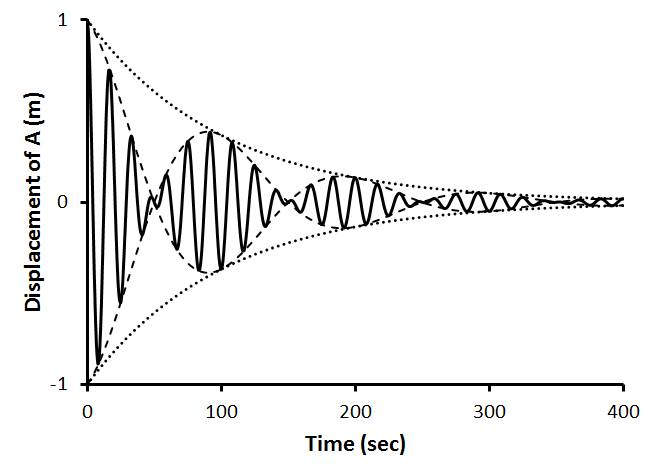
\includegraphics[width=7.2cm]{Figure01.png}\\
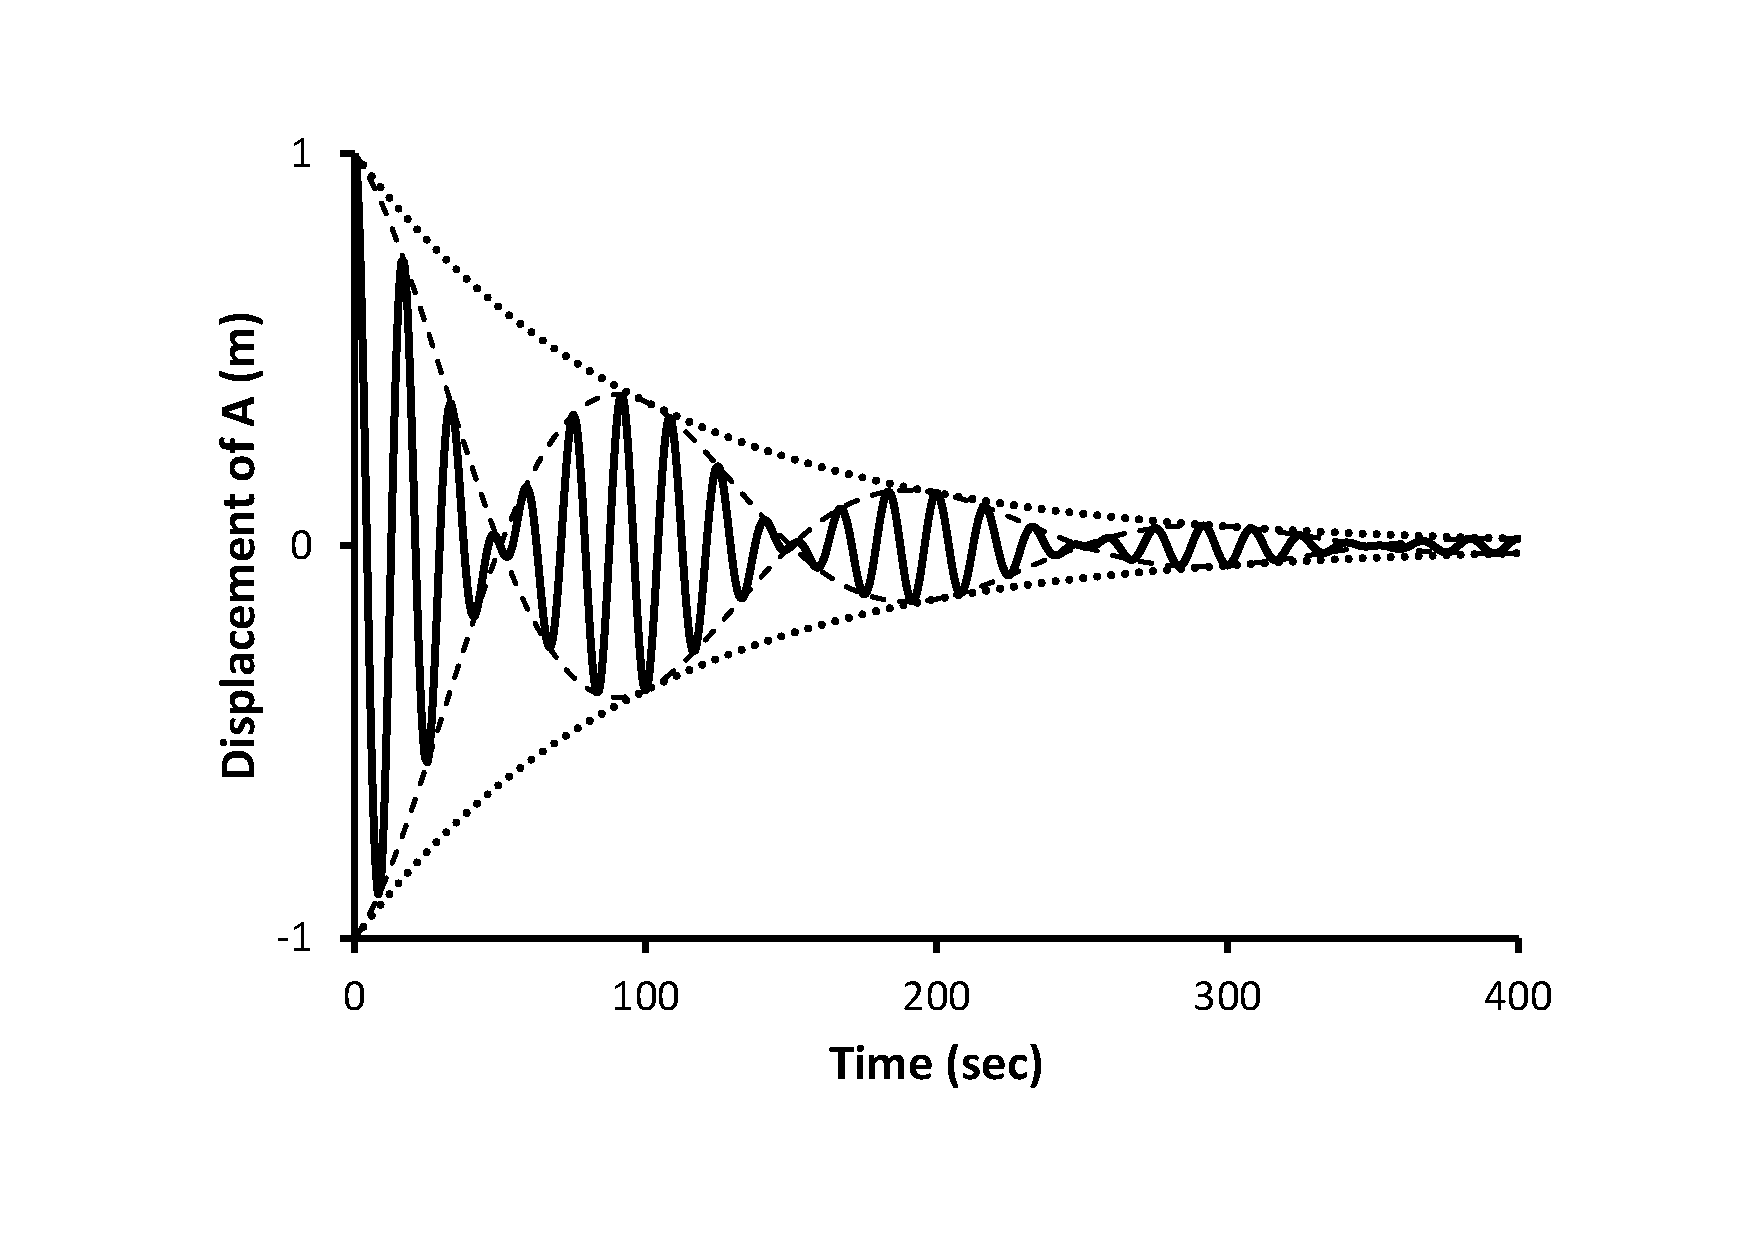
\includegraphics[width=9cm]{Figure01.pdf}
\caption{A linearly damped beat wave.} \label{Fig01}
\end{center}
\end{figure}

논문에 그림을 넣을 때 주의사항은 다음과 같다.
\begin{itemize}
\item{논문에 반드시 필요한 그림인가.}
\item{남들이 이해하는데 있어서 가장 알맞은 형태로 표현되었는가.}
\item{캡션과 본문에서의 설명은 충분한가.}
\end{itemize}
많은 학생들이 연구 과정에서 만들어진 사진들과 그래프들을 선별 과정 없이, 있는대로 다 넣으려는 경향을 보였다. 실험에서 사용한 장치들 사진이나 실험실 사진들을 넣는 경우도 있고, 연구 결과에서 텍스트 없이 그래프들만 나열시킨 경우도 있다. 따라서 십여장 남짓한 본문에서 텍스트가 차지하는 줄 수와 그림이 차지하는 줄 수를 비교하면, 그림의 점유 비율이 월등히 높은 논문들이 많았다. 원칙이 있는 건 아니지만, 글과 그림의 페이지 점유 정도를 비교할 때 글이 차지하는 비중을 높게 하도록 한다. 본인이 작성한 논문에서 그림의 양이 너무 많다면 그림의 양을 줄이고 글의 양을 늘려보자.

먼저 실험 장치 사진을 넣는 경우를 보자. 논문에서 실험 장치 사진을 넣는 것은 i) 장치 개발 자체가 연구 목적인 경우나 ii) 연구실에서 독자적으로 개발한 장치로 연구를 수행하기에 독자들이 연구 장치에도 호기심을 가질 것으로 판단되는 경우에만 필요한 것으로 굳이 필요한 상황이 아니라면 넣지 않도록 한다. 다만 연구 대상이 되는 물체의 상태 변화를 이해하기 쉽도록 그림으로 나타내는 과정에서 장치의 모식도가 함께 그려지는 경우는 종종 있다.

실험 결과를 충분한 텍스트 없이 그림만 나열하는 경우도 있다. 이 때는 그림들이 반드시 모두 들어가야 하는지 생각해본다. 각각의 그림들에 대해서 그림이 차지하는 공간 이상으로 글로 설명해야 할 내용이 있는지 생각해본다. 만약 여러 그림 중 하나만 대표가 선정되어 설명하게 된다면 나머지 그림들은 논문에서 불필요한 그림들이다. 그러나 모든 그림들을 종합하여 볼 필요가 있으며, 종합된 내용을 글로 설명해야 한다면 그림의 표현 방식이 잘못된 것이다. 이 때는 독자들에게 내용 전달에 있어서 효과적인 그림의 표현 방식이 어떤 것일지 고민을 해야 한다.

추가 : subfigure를 쓰는 방법에 대해 알아보자.

% example-image-a, example-image-b는 따로 이미지 파일이 존재하지 않아도 된다.
% http://tex.stackexchange.com/questions/130505/referencing-to-subfigures-in-main-caption 여기에 나와있는 큰 "A", "B" 그림이다. 혹시 에러로 인해 보이지 않는다면 참고. 
\begin{lstlisting}
	\begin{figure}[h]
	\centering
	\begin{subfigure}[t]{0.5\linewidth}
	\centering\includegraphics[width=100pt]{example-image-a}
	\caption{\label{subfig:fig1}}
	\end{subfigure}%
	\begin{subfigure}[t]{0.5\linewidth}
	\centering\includegraphics[width=100pt]{example-image-b}
	\caption{\label{subfig:fig2}}
	\end{subfigure}
	\caption{\subref{subfig:fig1} shows A and~\subref{subfig:fig2} shows B.}
	\label{subfigure_example}
	\end{figure}
\end{lstlisting}
\begin{figure}[h]
	\centering
	\begin{subfigure}[t]{0.5\linewidth}
		\centering\includegraphics[width=100pt]{example-image-a}
		\caption{\label{subfig:fig1}}
	\end{subfigure}%
	\begin{subfigure}[t]{0.5\linewidth}
		\centering\includegraphics[width=100pt]{example-image-b}
		\caption{\label{subfig:fig2}}
	\end{subfigure}
	\caption{\subref{subfig:fig1} shows A and~\subref{subfig:fig2} shows B.}
	\label{subfigure_example}
\end{figure}

동일한 맥락 상에서 그림이 여러 개일 경우 subfigure를 쓰게 된다. 위의 그림의 경우 `A' 라는 label 이 subfig:fig1, `B'라는 그림은 subfig:fig2, 전체 그림은 subfigure\_example 이다. 여기에서 \ref{subfig:fig1}, \subref{subfig:fig2}, \ref{subfigure_example} 등 여러 종류의 referencing을 하고 싶은데, 이는 Table \ref{table_subfigure_ref} 에 나타나 있다. 
\begin{table}[h]
	\caption{Subfigure에서 사용할 수 있는 여러 종류의 referencing.}
	\label{table_subfigure_ref}
	\centering
		\begin{tabular}{|c|c|}
		\hline
		명령어 & 결과 \\
		\hline
		\textbackslash ref\{subfig:fig1\} & \ref{subfig:fig1} \\
		\hline
		\textbackslash subref\{subfig:fig1\} & \subref{subfig:fig1} \\
		\hline
		\textbackslash ref\{subfigure\_example\} & 
		\ref{subfigure_example} \\
		\hline
	\end{tabular}
\end{table}

한 가지 주의해야 할 점은, \textbackslash subref\{\} 명령어는 여기에서는 (a) 와 같이 나타나지만, 기본 설정으로는 a 와 같이 나타난다는 점이다. gshs\_thesis.cls 를 사용하지 않는 다른 tex 문서에서 (a) 와 같이 나타내고 싶다면 다음과 같은 설정을 추가하면 된다.
\begin{quote}
	\textbackslash captionsetup\{subrefformat=parens\}
\end{quote}

추가 : 그림의 caption 이 길어질 경우, 이것이 List of Figures 에 그대로 실리게 될 경우 길어져서 가독성을 해칠 수 있다. 이럴 때는 다음과 같이 caption 에 List of Figures 에 실리게 될 내용만을 대괄호 안에 같이 적어 주면 된다. 
\begin{quote}
	\verb+\+caption[List of Figures 에 실리는 내용]\{본문에 실리는 내용\}
\end{quote}

\subsection{Tables}

\LaTeX에서 표를 넣는 방법은 i)엑셀 등 외부 프로그램에서 작성된 표를 pdf 그림파일로 변환하여 그림처럼 includegraphics 명령어로 넣는 방법 (물론 이 경우 {\textbackslash}begin\{figure\} 대신 {\textbackslash}begin\{table\}를 사용해야 함), ii)\LaTeX에서 표를 직접 제작하는 방법의 두 가지가 있다. \LaTeX에서는 명령어에 의해 표의 구획과 정렬, 선의 종류를 표현하므로 초보자에게는 다소 어려운 작업이 될 수 있다. 아마도 \LaTeX를 사용함에 있어서 가장 불편한 점은 표 제작 작업일 것이다. 다행히 인터넷에 `latex', `table' 등의 조합으로 검색하면 마우스로 제작한 표를 \LaTeX로 변환해주는 웹사이트들을 찾을 수 있다.

다음은 간단한 표의 예이다. 다음과 같이 입력을 하고 컴파일을 하면,
\begin{lstlisting}
	\begin{table}[h]
	\caption{Physical parameters.} \label{table01}
	\begin{center}
	\begin{tabular}{c|c|c}
	\hline
	& symbol & value \\ \hline
	Earth's mass & $M_E$ & $6.0\times 10^{24} {\rm kg}$ \\
	Earth's radius & $R_E$ & $6.4\times 10^6 {\rm m}$ \\
	Gravitational constant & $G$ & $6.67\times 10^{-11} {\rm N m^2 /kg^2}$ \\ \hline
	\end{tabular}
	\end{center}
	\end{table}
\end{lstlisting}
Table \ref{table01}과 같은 표를 얻게 된다.
\begin{table}[h]
	\caption{Physical parameters.}
	\label{table01}
	\centering
	\begin{tabular}{c|c|c}
	\hline
	 & symbol & value \\ \hline
	Earth's mass & $M_E$ & $6.0\times 10^{24} {\rm kg}$ \\
	Earth's radius & $R_E$ & $6.4\times 10^6 {\rm m}$ \\
	Gravitational constant & $G$ & $6.67\times 10^{-11} {\rm N m^2 /kg^2}$ 
	\\ \hline
	\end{tabular}
\end{table}

%주의사항 : 본 gshs\_thesis.tex 양식을 이용하여 표를 작성할 때는, 반드시 table 
%- center - tabular 환경을 사용해야 한다. 개인적인 성향에 따라 table 안에 
%\textbackslash centering 을 쓰고 tabular 환경을 사용할 수도 있지만, 이럴 경우 
%caption 이 표와 겹치는 결과를 불러일으킨다. 원인은 아직 밝혀지지 않았다.
%captionsetup의 skip 값이 음수였기 때문에 일어나는 문제였습니다. 수정되었습니다.

또한, figure의 경우 보통 그림 아래에 caption 이 붙지만, table의 경우 caption을 내용 위쪽에 붙여야 한다. 

본 양식은 졸업논문 양식의 advanced 버전으로, sub files를 사용한다. TeXstudio에서 사용할 경우 사용하는 모습은 그림 \ref{texstudio}와 같이, sub file들이 전부 나오고 클릭할 경우 파일이 열린다. TeXworks Editor에서는 상상도 못할 기능...
\begin{figure}
	\centering
	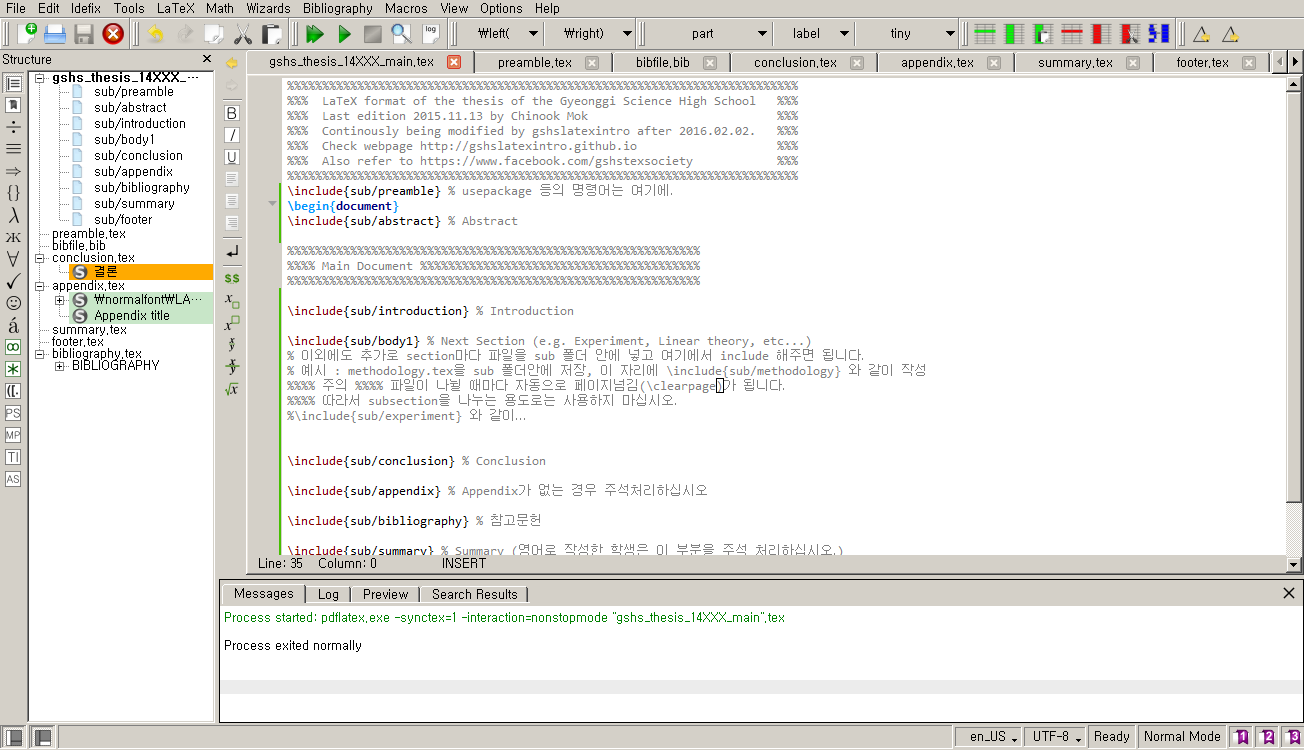
\includegraphics[width=\textwidth]{texstudio_struct.png}
	\caption{TeXstudio 에서 이 파일로 문서편집 하는 모습}
	\label{texstudio}
\end{figure}